\section{Operaci�n del sistema}

A continuaci�n, se presentan una serie de diagramas de secuencia que describen las interacciones entre las clases para ciertas funcionalidades.

En la \ref{fig:seq_load_visualization}, se presenta la secuencia de tareas que realiza la aplicaci�n desde que esta es abierta hasta que se visualiza la red.

Luego, en la \ref{fig:seq_simulation},  se muestra la serie de acciones realizadas para realizar la simulaci�n hidr�ulica utilizando los valores por defecto del archivo de red.

Finalmente, en la \ref{fig:seq_optimization}, se puede observar la interacci�n entre las clases de la aplicaci�n para poder llevar a cabo la resoluci�n de un problema, sea este monoobjetivo y multiobjetivo.

\begin{figure}[H]
    \centering
    \includegraphics[width=\textwidth]{Capitulo3/assets/sequence_load_visualization_network.eps}
    \caption{Diagrama de secuencia de la carga y visualizaci�n de la red.}
    \label{fig:seq_load_visualization}
\end{figure}

\begin{figure}[H]
    \centering
    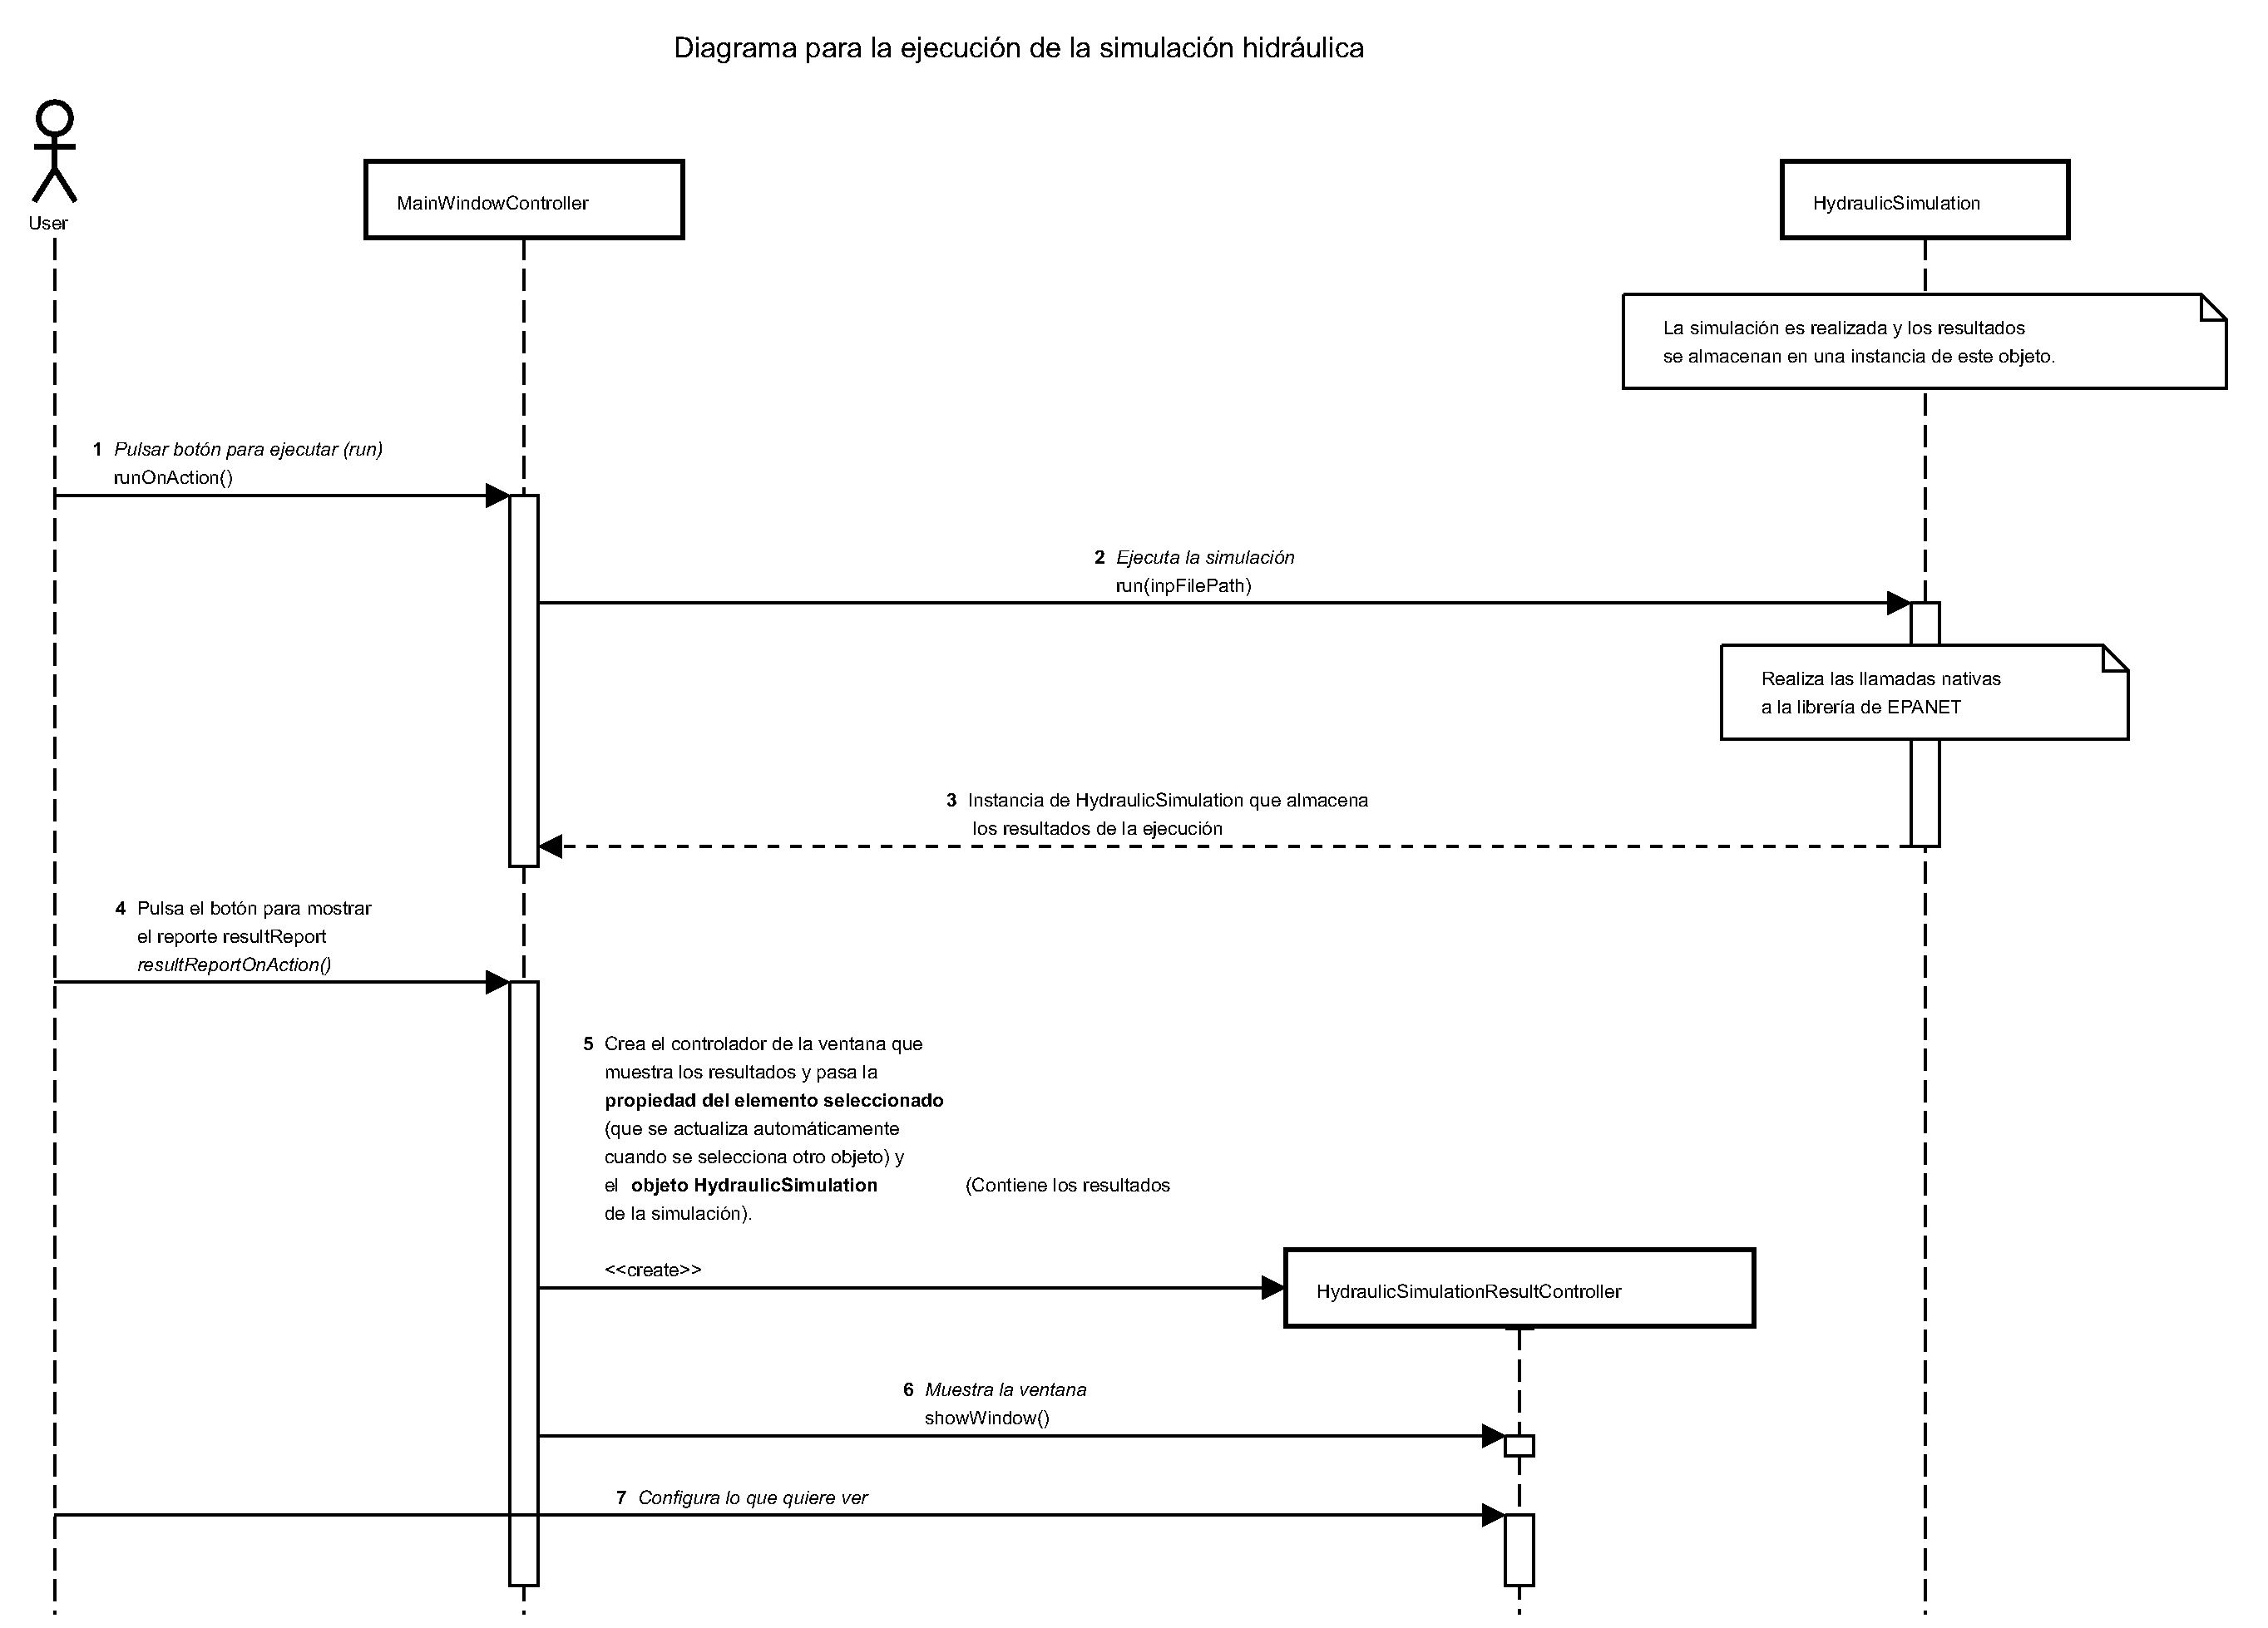
\includegraphics[width=\textwidth]{Capitulo3/assets/sequence_hydraulic_simulation.eps}
    \caption{Diagrama de secuencia de la simulaci�n de la red usando los valores del archivo de configuraci�n de red (inp).}
    \label{fig:seq_simulation}
\end{figure}

\begin{figure}[H]
    \centering
    \includegraphics[width=\textwidth]{Capitulo3/assets/sequence_optimization.eps}
    \caption{Diagrama de secuencia de la optimizaci�n.}
    \label{fig:seq_optimization}
\end{figure}